\documentclass{beamer}
%\documentclass[handout]{beamer}

% language settings
%\usepackage{fontspec, polyglossia}
%\setdefaultlanguage{magyar}

% common packages
\usepackage{amsmath, multimedia, hyperref, color, multirow}
%\usepackage{graphicx}

% TikZ
\usepackage{tikz}
%\usetikzlibrary{arrows.meta, decorations.pathmorphing, decorations.pathreplacing, shapes.geometric,mindmap}
\usetikzlibrary{shapes.geometric}

% beamer styles
\mode<presentation>{
\usetheme{CambridgeUS}
\usecolortheme{dove}
%\usefonttheme{structureitalicserif}
\setbeamercovered{transparent}
}
\setbeamertemplate{blocks}[rounded][shadow=true]

\AtBeginSection[]{
  \begin{frame}<beamer>{Contents}
    %\tableofcontents[currentsection]
    \tableofcontents[currentsection,currentsubsection]
  \end{frame}
}
\useoutertheme[]{miniframes}

% title, etc
\title{Characterization of 5+ Callers}
%\subtitle{A subtitle may be shorter and more technical}
\author{Attila Jones, Chaggai Rosenbluh, Andy Chess}
\date{Mount Sinai, New York}

\begin{document}

\maketitle

\section{Introduction}

\begin{frame}<1>[label=workflow]{Our workflow}
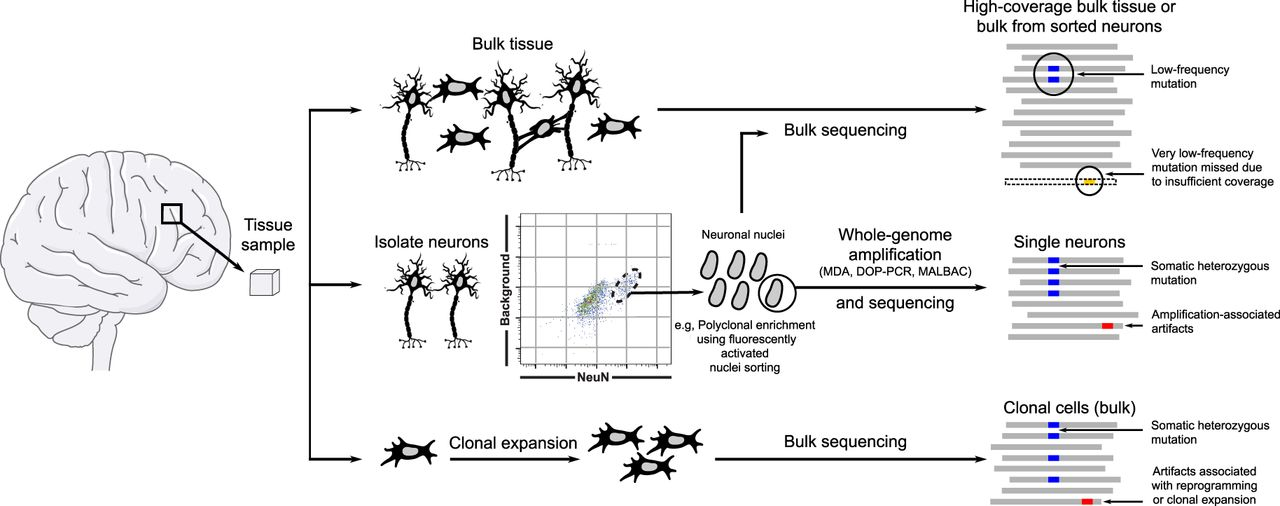
\includegraphics[width=0.8\textwidth]{figures/from-others/bsm-science-fig2.jpg}
\small
\begin{enumerate}
\item brain sample
\begin{itemize}
\item MosaicForecast (Park Lab, unpublished), strelka2Germline
\end{itemize}
\item<2> brain + control sample
\begin{itemize}
\item lofreqSomatic, MuTect2, strelka2Somatic, somaticSniper
\end{itemize}
\end{enumerate}
\end{frame}


\begin{frame}{Spread of somatic mosaicism}
\includegraphics[height=0.7\textheight]{figures/from-others/lodato2015science-fig3b.png}
\vfill
\tiny{Lodato et al Science 2015}
\end{frame}

\againframe<2>{workflow}

\begin{frame}[label=precrecall]{Measuring performance of somatic variant calling}
%{Compare call set \(C\) to truth set \(V\)}
\begin{description}
\item [\(C\)] some call set of somatic variants
\item [\(V\)] the truth set of somatic variants
\begin{enumerate}
\item validation experiment
\item mixing experiment
\end{enumerate}
\end{description}
\vfill
\alert{Precision}\\
the fraction of calls that are true
\begin{equation}
p(C) = \frac{|C \cap V|}{|C|} = \frac{\#\text{true calls}}{\#\mathrm{calls}}
\end{equation}
\alert{Recall}\\
the fraction of variants that are called
\begin{equation}
r(C) = \frac{|C \cap V|}{|V|} = \frac{\#\text{true calls}}{\#\mathrm{variants}}
\end{equation}
\end{frame}

\section{Validation experiment}

\begin{frame}{Experimental validation}
\includegraphics[scale=0.8]{../../notebook/2019-07-23-commonsample-precrecall/named-figure/prec-recall-common-sample-mosaicforecast.pdf}
\end{frame}

\section{Mixing experiment}

\begin{frame}{Mixing experiment}
\begin{columns}[t]
\begin{column}{0.5\textwidth}

\includegraphics[scale=0.3]{../../notebook/2018-05-01-ceph-vars-greally/figure/venn-S1-1.pdf}
\end{column}

\begin{column}{0.5\textwidth}

{\footnotesize
{\large mixing proportions}

\begin{tabular}{r|ccc}
genome & mix1 & mix2 & mix3 \\
\hline
NA12889 & 4 & 2 & 0 \\
NA12891 & 8 & 4 & 0 \\
NA12890 & 16 & 8 & 0 \\
NA12892 & 72 & 86 & 100 \\
& & & \\
\end{tabular}
}
\end{column}
\end{columns}
\end{frame}

\begin{frame}{Allele frequency}
\begin{columns}[t]
\begin{column}{0.5\textwidth}

{\tiny
\begin{tabular}{c|ccc}
genotype & \multicolumn{3}{c}{AAF (\%)} \\
& mix1 &  mix2 & mix3 \\
\hline
0001 & 36 & 43 & 50\\
0010 & 8 & 4 & 0\\
0100 & 4 & 2 & 0\\
1000 & 2 & 1 & 0\\
0002 & 72 & 86 & 100\\
... & ... & ... & ...\\
2212 & 92 & 96 & 100\\
2221 & 64 & 57 & 50\\
2222 & 100 & 100 & 100\\
\end{tabular}
}

\includegraphics[width=1.0\columnwidth]{../../notebook/2019-04-24-vaf-model-taejeong/named-figure/tj-vaf-hist-expon-pooled.pdf}

\end{column}

\begin{column}{0.5\textwidth}

\includegraphics[width=1.0\columnwidth]{../../notebook/2019-04-04-truth-sets-aaf/named-figure/vaf-mix1-vaf.pdf}

\includegraphics[width=1.0\columnwidth]{../../notebook/2019-04-04-truth-sets-aaf/named-figure/exp-model0-lam02-mix1.pdf}
\end{column}
\end{columns}
\end{frame}

\begin{frame}{Performance: SNVs}
\includegraphics[width=0.8\textwidth]{../../notebook/2019-08-15-benchmark-calls/named-figure/prec-recall-snp-region-autosomes-mix3_ctr.pdf}
\end{frame}

\begin{frame}{Discrepancy: MosaicForecast}
\begin{columns}[t]
\begin{column}{0.5\textwidth}

validation experiment

\includegraphics[width=1.0\columnwidth]{../../notebook/2019-07-23-commonsample-precrecall/named-figure/prec-recall-common-sample-mosaicforecast.pdf}
\end{column}
\begin{column}{0.5\textwidth}

mixing experiment

\includegraphics[width=1.0\columnwidth]{../../notebook/2019-08-15-benchmark-calls/named-figure/prec-recall-snp-region-autosomes-mix3_ctr.pdf}
\end{column}
\end{columns}
\end{frame}

\begin{frame}{Effect of control sample}
\includegraphics[scale=0.45]{../../notebook/2019-08-15-benchmark-calls/named-figure/prec-recall-controlsample-effect.pdf}
\end{frame}

\begin{frame}[label=familyoftruthsets]{A family of truth sets}
\includegraphics[width=0.85\textwidth]{../../notebook/2019-04-04-truth-sets-aaf/named-figure/exp-model-mix1.pdf}
{\tiny
\begin{tabular}{c|r|r}
s2g & SNV & indel \\
\hline
-4 & 400 & 80 \\
-3 & 4000 & 800 \\
-2 & 40000 & 8000 \\
\end{tabular}
}
\end{frame}

\begin{frame}{Effect of number of somatic variants}
\includegraphics[scale=0.45]{../../notebook/2019-08-15-benchmark-calls/named-figure/prec-recall-s2g-effect.pdf}
\end{frame}

\againframe{familyoftruthsets}

\begin{frame}{Effect of allele frequency distribution}
\includegraphics[scale=0.45]{../../notebook/2019-08-15-benchmark-calls/named-figure/prec-recall-lambda-effect.pdf}
\end{frame}

\section{Callset combination and filtering}

\begin{frame}{Why combine callers with machine learing?}
\begin{itemize}
\item no best universal caller
\begin{itemize}
\item precision
\item VAF in brain (and control) sample
\end{itemize}
\item callers don't provide the single best way of ranking calls
\item much info in quality annotations on calls
\end{itemize}
\end{frame}

\begin{frame}
\begin{columns}[t]
\begin{column}{0.3\textwidth}
\small
callset \(j\):

\(\{\overbrace{y_{i}}^\text{label},
\overbrace{\mathbf{x}_{ij}}^\text{annot}\}_{i=1,...,n_j}\)
\end{column}

\begin{column}{0.7\textwidth}

{\small

\tikz[baseline=-0.5ex] \path (0,0) -- node[draw, fill=blue, circle, inner
sep=2.5pt] {} (1,0); false positive: \(y_{ij}=0\)

\tikz[baseline=-0.5ex] \path (0,0) -- node[draw, fill=red, rectangle, inner
sep=3.0pt] {} (1,0); true positive: \(y_{ij}=1\)

\tikz[baseline=-0.5ex] \path (0,0) -- node[draw, diamond, inner
sep=3.0pt] {} (1,0); unlabeled: \(y_{ij}=?\)
}
\end{column}
\end{columns}
\begin{columns}[t]
\begin{column}{0.5\textwidth}
\end{column}

\begin{column}{0.5\textwidth}

\end{column}
\end{columns}
\begin{columns}[t]
\begin{column}{0.33\textwidth}
\begin{center}
\(j=1\)
\end{center}

\includegraphics[width=1\columnwidth]{figures/by-me/vcf-annot-classif/strelka2/strelka2-unlabeled.pdf}
\end{column}

\begin{column}{0.33\textwidth}
\begin{center}
\(j=...\)

\vspace{0.7in}
\large
\(\cdots\)
\normalsize
\end{center}
\end{column}

\begin{column}{0.33\textwidth}
\begin{center}
\(j=5\)
\end{center}

\includegraphics[width=1\columnwidth]{figures/by-me/vcf-annot-classif/tnseq/tnseq-unlabeled.pdf}
\end{column}
\end{columns}
\end{frame}


\begin{frame}
\small
\begin{center}
Probability that a call is true
\(
P(i) = \frac{1}{5} \sum_{j=1}^5 P_j(y_{ij} | \mathbf{x}_{ij})
\)
\end{center}
\begin{columns}[t]
\begin{column}{0.33\textwidth}
\begin{center}
\(j=1\)
\end{center}

\includegraphics[width=1\columnwidth]{figures/by-me/vcf-annot-classif/strelka2/strelka2-svm-unlabeled.pdf}
\end{column}

\begin{column}{0.33\textwidth}
\begin{center}
\(j=...\)

\vspace{0.7in}
\large
\(\cdots\)
\normalsize
\end{center}
\end{column}

\begin{column}{0.33\textwidth}
\begin{center}
\(j=5\)
\end{center}

\includegraphics[width=1\columnwidth]{figures/by-me/vcf-annot-classif/tnseq/tnseq-svm-unlabeled.pdf}
\end{column}
\end{columns}
\end{frame}


\begin{frame}{VariantMetaCaller}{Gezsi et al 2015 BMC Genomics}
\includegraphics[scale=0.8]{../../notebook/2019-08-15-benchmark-calls/named-figure/prec-recall-vmc-s2g-3.pdf}
\end{frame}

%\againframe{precrecall}

\begin{frame}{Summary}
\begin{itemize}
\item callers' relative performance depends on
\begin{itemize}
\item benchmark data and truth set
\item variant allele frequency (VAF) in brain and control sample
\item distribution of VAF across variants
\end{itemize}
\item notable
\begin{itemize}
\item MosaicForecast: the best under several conditions 
\item lofreqSomatic, strelka2Somatic, MuTect2: strong performance when control sample lacks variant 
\item strelka2Germline: only useful for at high VAF
\end{itemize}
\item combining multiple callsets
\begin{itemize}
\item machine learning (VariantMetaCaller)
\item high performance
\item precision based filtering 
\end{itemize} 
\end{itemize}
\end{frame}

\begin{frame}{Acknowledgements}
\begin{columns}[t]
\begin{column}{0.5\textwidth}
\alert{Akbarian Lab, Mount Sinai}

\vspace{1em}
\alert{Park Lab, Harvard}

\emph{Yanmei Dou} (MosaicForecast)

\vspace{1em}
\alert{Walsh Lab, Harvard}

\vspace{1em}
\alert{Urban Lab, Stanford}

\emph{Xiaowei Zhu} (RetroSom)

\end{column}

\begin{column}{0.5\textwidth}
\end{column}
\end{columns}
\end{frame}

\end{document}



\begin{columns}[t]
\begin{column}{0.5\textwidth}

\end{column}

\begin{column}{0.5\textwidth}

\end{column}
\end{columns}
